\begin{apendicesenv}

\partapendices

\chapter{Instruções para preenchimento do questionário}
\label{apen-inst}
Caros,

O estudo a seguir faz parte de uma pesquisa realizada por um aluno de Engenharia de \emph{software}, da Universidade de Brasília – \textbf{UnB}, o qual será utilizado como forma de obtenção de conhecimento sobre o tema.

Esta pesquisa visa investigar se os alunos da Universidade de Brasília utilizam as redes sociais, como o \textit{Facebook}, para o compartilhamento de recursos e informações relacionados as disciplinas cursadas na Universidade. Para tanto, necessito de sua colaboração respondendo ao questionário sobre o tema. É importante ressaltar que os dados aqui levantados serão compilados e utilizados apenas para fins acadêmicos, na problematização da pesquisa.

Instruções para preenchimento do questionário:
\begin{enumerate}
\item Você deverá selecionar um item para indicar o grau de concordância com as assertivas apresentadas na tabela \ref{tab:preenchimento}.

\begin{table}[h]
\center
\begin{tabular}{|c|c|c|c|c|}
\hline
		\textbf{NUNCA} & \textbf{RARAMENTE} & \textbf{ÀS VEZES} & \textbf{FREQUENTEMENTE} & \textbf{SEMPRE}\\ \hline
\end{tabular}
\caption{Opções para preenchimento do questionário.}
\label{tab:preenchimento}
\end{table}
\textbf{Lembrando} que quanto mais próximo de \textbf{Nunca}, \textbf{MENOR} o grau de concordância. Quanto mais próximo de \textbf{Sempre}, \textbf{MAIOR} o grau de concordância.

\item O questionário deve ser respondido pelos alunos das Universidade de Brasília;

\item Não existem respostas "certas" ou "erradas". O importante é respondê-las de forma \textbf{sincera}.

\item Procure não deixar nenhuma resposta em branco. Sua participação é muito importante para a finalização deste trabalho.
\end{enumerate}

Desde já agradeço sua atenção e cooperação. Coloco-me à disposição para os esclarecimentos que se fizerem necessários.

Cordialmente,
\begin{description}
\item Hebert Douglas de Almeida Santos <hebertdougl@gmail.com>
\end{description}

\chapter{Questionário para problematização}
\label{apen-quest}

\begin{enumerate}
% \item \label{itm-first} Você utiliza algum tipo de rede social para uso pessoal?

\item \label{pergunta1} Com que frequência você utiliza redes sociais?

\item \label{pergunta2} Você utiliza alguma rede social como ferramenta de apoio as disciplinas?

\item \label{pergunta3} Os professores incentivam o uso de redes sociais para suas disciplinas?

\item \label{pergunta4} Mesmo que o professor não recomende o uso de redes sociais para discussão de conteúdos de suas disciplinas, você as utiliza?

\end{enumerate}


\chapter{Avaliação dos resultados}
\label{apen-quest-result}

\begin{figure}[h]
    \centering
    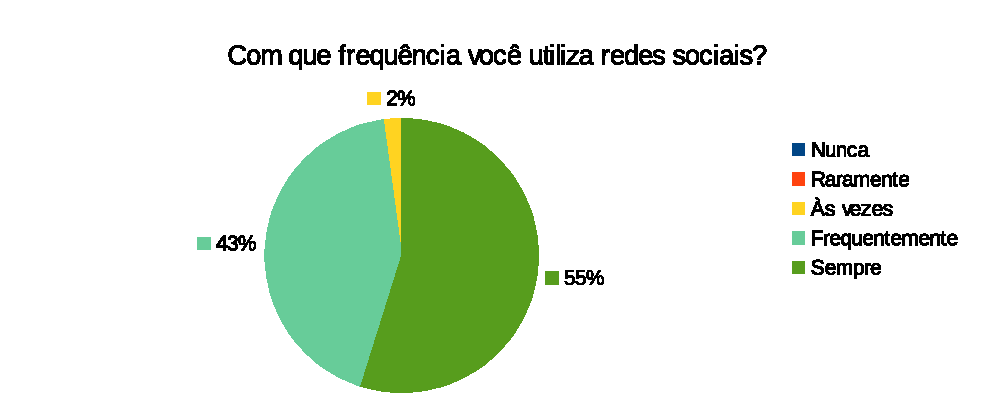
\includegraphics[keepaspectratio=true,scale=0.55]
      {figuras/pergunta1p.eps}
    \caption{Resultados do questionário para a pergunta \ref{pergunta1}}
    \label{pergunta1}
\end{figure}

\begin{figure}[h]
    \centering
    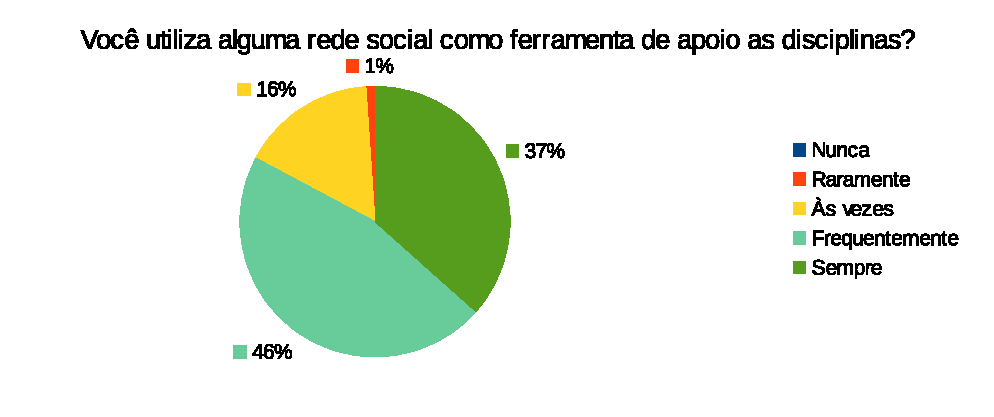
\includegraphics[keepaspectratio=true,scale=0.55]
      {figuras/pergunta2p.eps}
    \caption{Resultados do questionário para a pergunta \ref{pergunta2}}
    \label{pergunta2}
\end{figure}

\begin{figure}[h]
    \centering
    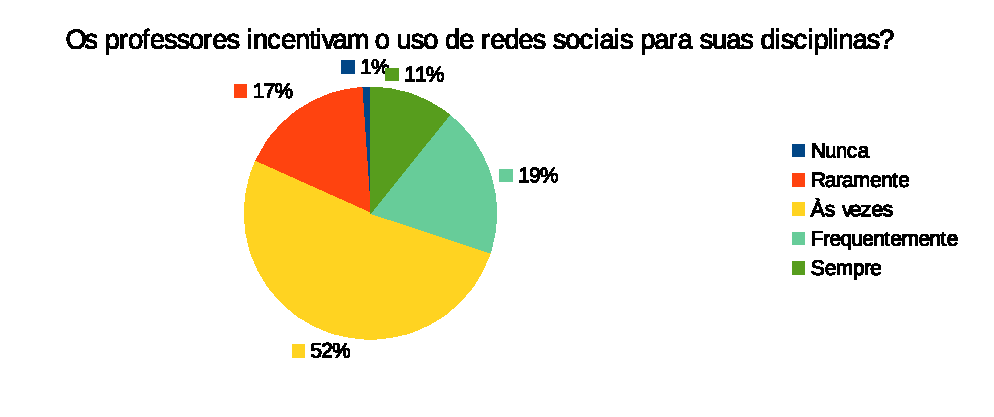
\includegraphics[keepaspectratio=true,scale=0.55]
      {figuras/pergunta3p.eps}
    \caption{Resultados do questionário para a pergunta \ref{pergunta3}}
    \label{pergunta3}
\end{figure}

\begin{figure}[h]
    \centering
    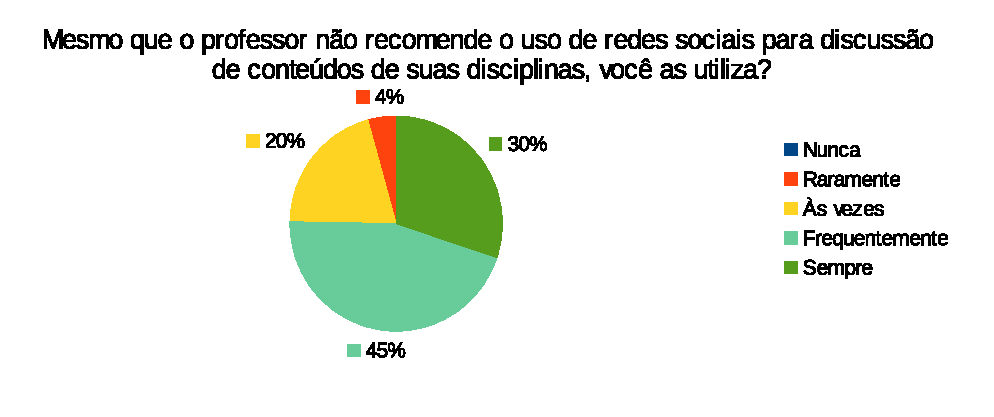
\includegraphics[keepaspectratio=true,scale=0.55]
      {figuras/pergunta4p.eps}
    \caption{Resultados do questionário para a pergunta \ref{pergunta4}}
    \label{pergunta4}
\end{figure}

\end{apendicesenv}